%%%%%%%%%%%%%%%%%%%%%%%%%%%%%%%%%%%%%%%%%
% Jacobs Portrait Poster
% LaTeX Template
% Version 1.0 (31/08/2015)
% (Based on Version 1.0 (29/03/13) of the landscape template
%
% Created by:
% Computational Physics and Biophysics Group, Jacobs University
% https://teamwork.jacobs-university.de:8443/confluence/display/CoPandBiG/LaTeX+Poster
% 
% Further modified by:
% Nathaniel Johnston (nathaniel@njohnston.ca)
%
% Portrait version by:
% John Hammersley
%
% The landscape version of this template was downloaded from:
% http://www.LaTeXTemplates.com
%
% License:
% CC BY-NC-SA 3.0 (http://creativecommons.org/licenses/by-nc-sa/3.0/)
%
%%%%%%%%%%%%%%%%%%%%%%%%%%%%%%%%%%%%%%%%%

%----------------------------------------------------------------------------------------
%	PACKAGES AND OTHER DOCUMENT CONFIGURATIONS
%----------------------------------------------------------------------------------------

\documentclass[final]{beamer}

\usepackage[scale=1]{beamerposter} % Use the beamerposter package for laying out the poster
\usepackage{xcolor}
\usepackage{amsmath}
\usepackage{amssymb}
\usepackage{siunitx}
\usepackage{braket}
\usepackage{bbold}
\usepackage{bigints}
\usepackage{mathtools}
\usepackage{bm}

\sisetup{detect-all,mode=math,math-rm=\mathrm}

\definecolor{ubcblue}{cmyk}{1,0.9,0.13,0.68}
\definecolor{ubcblue1}{cmyk}{1,0.68,0.04,0}
\definecolor{ubcblue2}{cmyk}{0.8,0.12,0.01,0}
\definecolor{ubcblue3}{cmyk}{0.64,0.1,0.01,0}
\definecolor{ubcblue4}{cmyk}{0.52,0.05,0.03,0}
\definecolor{ubcblue5}{cmyk}{0.38,0.02,0.05,0}

\usetheme{confposter} % Use the confposter theme supplied with this template

\setbeamercolor{block title}{fg=ubcblue,bg=white} % Colors of the block titles
\setbeamercolor{block body}{fg=black,bg=white} % Colors of the body of blocks
\setbeamercolor{block alerted title}{fg=white,bg=ubcblue} % Colors of the highlighted block titles
\setbeamercolor{block alerted body}{fg=black,bg=white} % Colors of the body of highlighted blocks
% Many more colors are available for use in beamerthemeconfposter.sty

%-----------------------------------------------------------
% Define the column widths and overall poster size
% To set effective sepwid, onecolwid and twocolwid values, first choose how many columns you want and how much separation you want between columns
% In this template, the separation width chosen is 0.024 of the paper width and a 4-column layout
% onecolwid should therefore be (1-(# of columns+1)*sepwid)/# of columns e.g. (1-(4+1)*0.024)/4 = 0.22
% Set twocolwid to be (2*onecolwid)+sepwid = 0.464
% Set threecolwid to be (3*onecolwid)+2*sepwid = 0.708

\newlength{\sepwid}
\newlength{\onecolwid}
\newlength{\twocolwid}
\newlength{\threecolwid}
\setlength{\paperwidth}{36in} % A0 width: 46.8in
\setlength{\paperheight}{48in} % A0 height: 33.1in
\setlength{\sepwid}{0.024\paperwidth} % Separation width (white space) between columns
%\setlength{\onecolwid}{0.22\paperwidth} % Width of one column
%\setlength{\twocolwid}{0.464\paperwidth} % Width of two columns
%\setlength{\threecolwid}{0.708\paperwidth} % Width of three columns
\setlength{\onecolwid}{0.3013\paperwidth} % Width of one column
\setlength{\twocolwid}{0.6267\paperwidth} % Width of two columns
\setlength{\topmargin}{-0.5in} % Reduce the top margin size
%-----------------------------------------------------------

\usepackage{graphicx}  % Required for including images

\usepackage{booktabs} % Top and bottom rules for tables
\usepackage{eso-pic}

%----------------------------------------------------------------------------------------
%	TITLE SECTION 
%----------------------------------------------------------------------------------------

\title{Large Zero Bias Conductance Peak \\in Dirac Semimetal-Superconductor Devices}

\author{\underline{R. Haenel}\inst{1}, \underline{W. Yu}\inst{2}, M.A.
	Rodriguez\inst{2}, S.R. Lee\inst{2}, F. Zhang\inst{4}, M. Franz\inst{1}, D. I. Pikulin\inst{5}, and W. Pan\inst{2,3}} % Author(s)

\institute{
	\inst{1} Stewart Blusson Quantum
	Matter Institute, University of British Columbia, Vancouver \quad
	\inst{2} Sandia National Laboratories, Albuquerque, New Mexico \\
	\inst{3} Sandia National Laboratories, Livermore, California \quad
	\inst{4} University of Texas at Dallas \quad
\inst{5}Microsoft Station Q, University of California, Santa Barbara} % Institution(s)
%----------------------------------------------------------------------------------------

\usepackage{exscale}
\begin{document}

\newcommand\AtPagemyLowerLeft[1]{\AtPageLowerLeft{%
\put(\LenToUnit{0.805\paperwidth},\LenToUnit{0.957\paperheight}){#1}}}
\newcommand\AtPagemyLowerRight[1]{\AtPageLowerLeft{%
\put(\LenToUnit{0.014\paperwidth},\LenToUnit{0.953\paperheight}){#1}}}
\AddToShipoutPictureFG{
  \AtPagemyLowerLeft{{
\includegraphics[width=17cm,keepaspectratio]{fig/logos3}}}
}%
\AddToShipoutPictureFG{
	\AtPagemyLowerRight{{
\includegraphics[width=10.5cm,keepaspectratio]{fig/ubc_qmi}}}
}%


\addtobeamertemplate{block end}{}{\vspace*{2ex}} % White space under blocks
\addtobeamertemplate{block alerted end}{}{\vspace*{2ex}} % White space under highlighted (alert) blocks

\setlength{\belowcaptionskip}{2ex} % White space under figures
\setlength\belowdisplayshortskip{2ex} % White space under equations

\begin{frame}[t] % The whole poster is enclosed in one beamer frame

\begin{columns}[t] % The whole poster consists of three major columns, the second of which is split into two columns twice - the [t] option aligns each column's content to the top

\begin{column}{\sepwid}\end{column} % Empty spacer column

\begin{column}{\onecolwid} % The first column

%----------------------------------------------------------------------------------------
%	OBJECTIVES
%----------------------------------------------------------------------------------------

\begin{alertblock}{Summary}
We report the observation of a large ZBCP in superconducting junction structures mediated by 
surface states of the Dirac semimetal Cd$_3$As$_2$. Our detailed analyses
suggest that this large ZBCP is most likely not caused by MZMs. We attribute it,
instead, to the existence of a supercurrent between two far-separated
superconducting Al electrodes.
\end{alertblock}

%----------------------------------------------------------------------------------------
%	INTRODUCTION
%----------------------------------------------------------------------------------------

\begin{block}{Introduction}
	Majorana zero modes (MZMs) are widely seen as a promising
	route towards the realization of topological quantum computation. One of
	the experimental hallmarks of the presence of MZMs is 
	a quantized zero bias conductance peak (ZBCP) in differential
	conductance measurements. Here, we report the observation of such a large
	ZBCP in Fig. \ref{fig:exp} in transport measurements across a
	Ti/Au-Cd$_3$As$_2$-Al junction.

%------------------------------------------------

\begin{figure}
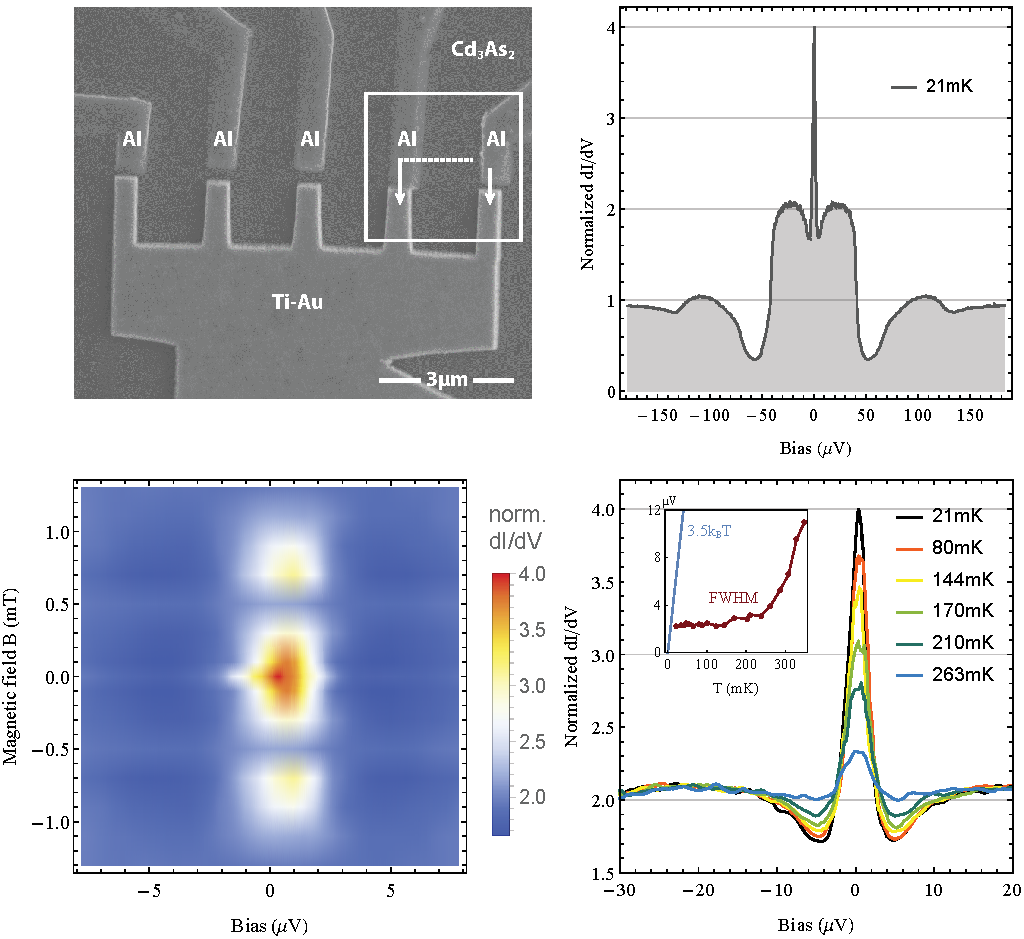
\includegraphics[width=\linewidth]{fig/figure1.pdf}
\caption{\sffamily \, Device geometry and temperature and magnetic field dependence
	of differential conductance measured across the rightmost junction.}
\label{fig:exp}
\end{figure}

The upper right panel of Fig. \ref{fig:exp} shows the differential conductance
at 21 mK. The normal state conductance roughly doubles at
around 50\text{$\mu$}V as a result of perfect Andreev reflection.
This indicates that a very clean interface between Cd$_3$As$_2$ and the
superconducting Al electrode has been
fabricated and a that gap $\Delta$ has been induced by proximity of the Al electrode. At zero bias, a
sharp peak is present. The bottom panels show its magnetic field- and
temperature-dependence.

\end{block}
%----------------------------------------------------------------------------------------


\begin{block}{Model}
We model the Dirac semimetal Cd$_3$As$_2$ by the effective low energy theory
\begin{equation}
	\label{eqn:ham}
  H_0(\mathbf{k})=\varepsilon(\mathbf{k}) + 
  \begin{pmatrix}
    M(\mathbf{k}) & A k_- & 0 & 0\\
    A k_+ & -M(\mathbf{k}) & 0 & 0\\
    0 & 0 & -M(\mathbf{k}) & -Ak_-\\
    0 & 0 & -A k_+ & M(\mathbf{k})
  \end{pmatrix}
\end{equation}
where $k_\pm = k_x \pm i k_y$ and $M(\mathbf{k})$, $\varepsilon(\mathbf{k})$ are
even functions in $\mathbf{k}$ \cite{Wang2013}. 


\end{block}
\begin{figure}
	\includegraphics[width=0.75\linewidth]{fig/band.pdf}
	\caption{\sffamily \, Bandstructure for Hamiltonian (\ref{eqn:ham}) with finite
	$L_x/a_x=80$. }
\label{fig:band}
\end{figure}

\end{column} % End of the first column

\begin{column}{\sepwid}\end{column} % Empty spacer column

\begin{column}{\onecolwid} % Begin a column (column 2)
\rmfamily
\justify
To model the junction
geometry, we regularize the Hamiltonian on a lattice and add a spatially dependent superconducting order
parameter $\Delta$ to obtain the BdG-Hamiltonian
\begin{eqnarray*}
	H = \begin{pmatrix}
		H_0 -\mu& \Delta(x) \\
	\Delta^*(x) & -\left(\mathcal{T}H_0\mathcal{T}^{-1} -\mu\right)
\end{pmatrix} \,.
\end{eqnarray*}
$\mathcal{T}$ is the time-reversal operation with $\mathcal{T}^2=-1$, $\mu$ is
the chemical potential. In numerical simulations, we further add terms that are
consistent with symmetry class DIII.

\begin{block}{Majorana zero modes}

\begin{figure}
	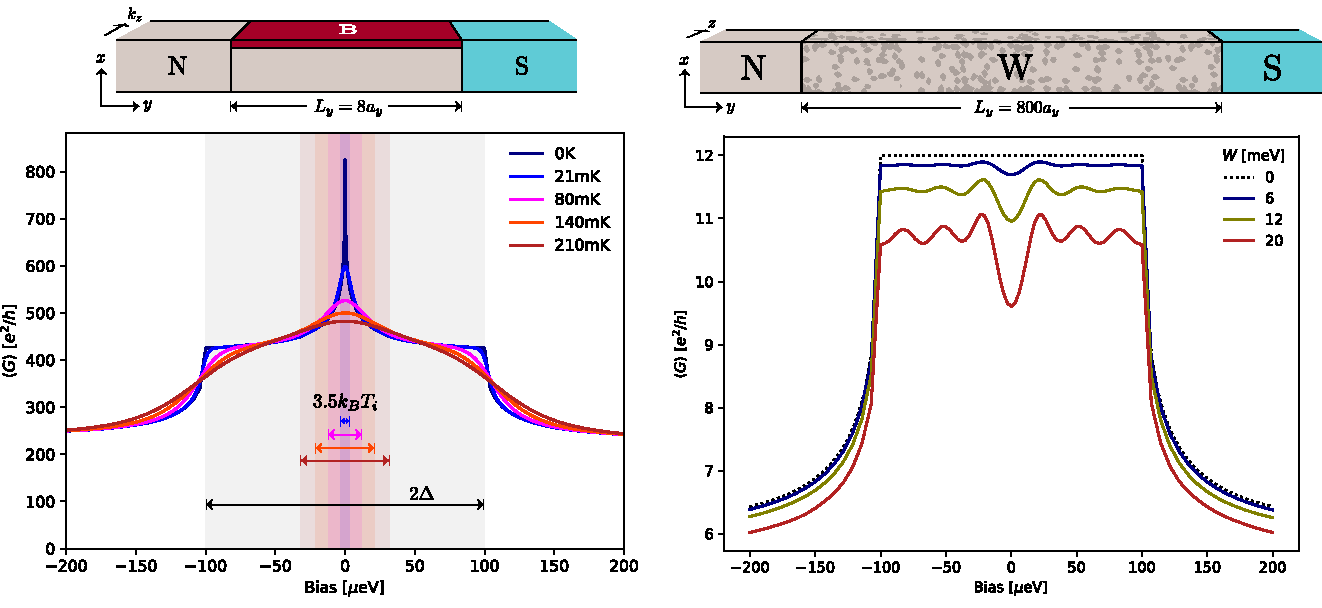
\includegraphics[width=\linewidth]{fig/transport.pdf}
	\caption{\sffamily \, Transport simulations in the presence of a magnetic gap (left)
	and for disorder that couples QSHI for different $k_z$ averaged over 40
	realizations of disorder (right). N
	denotes the normal lead, S denotes the superconducting lead. The
conductance dip is consistent with Weak Localization.}
\label{fig:transport}
\end{figure}

When $k_z$ in Eq. (\ref{eqn:ham}) is treated as a parameter, the
	Hamiltonian describes a 2D Quantum Spin Hall insulator (QSHI). The
	low-energy field theory of such a QSHI is identical to the low energy
	description of the Kitaev chain which exhibits MZMs localized at its ends.
	The QSHI edge states do not have ends. However, MZMs are found at
	boundaries to gapped regions. Since backscattering between the edge
	states of a single QSHI is forbidden by $\mathcal{T}$, 
	we can most easily create a gap by
	breaking time-reversal symmetry. A quantum transport simulation for such
	a scenario is shown in the left panel of Fig. \ref{fig:transport}. 
	
	A second way to create a gap and to localize MZMs 
	involves backscattering between
	QSHI of different $k_z$. However, this approach
	requires fine-tuning since such
	scattering processes can hybridize MZMs at different $k_z$. We were not
	able to find a suitable parameter regime and instead observed a zero-bias
	dip consistent with Weak Localization, in disagreement to the
	experiment.

\end{block}

\begin{block}{ZBCP due to supercurrent}
	Finite-temperature smearing should yield a ZBCP of width $3.5k_B T$, as
	exemplified in the left panel of Fig. \ref{fig:transport}. However, the experimentally
	observed width is much smaller (see inset of bottom right panel in
	Fig. \ref{fig:exp}). This strongly suggests that the ZBCP 
	is not caused by any
	single-particle mechanism.

	Consequently, we investigate the scenario of an additional 
	supercurrent channel that
	exists between two neighboring Al-electrodes, next to the
	conductance channel of the NS junction. The IV
	relationship for a Josephson junction 
	in the presence of thermal Nyquist noise has been derived
	in \cite{Ivanchenko},



\begin{eqnarray}
	\label{eqn:zilberman}
  I(V) = I_0 \text{Im} \left[\frac{I_{1-2 i \beta (V + R_2 I) \hbar/(2e
  (R_1+R_2))}(\beta \frac{\hbar}{2e}I_0 \frac{\Delta(T)}{\Delta(0)})}{I_{-2 i
  \beta (V + R_2 I) \hbar/(2e (R_1+R_2))}(\beta \frac{\hbar}{2e}I_0
  \frac{\Delta(T)}{\Delta(0)})}\right] \,.
\end{eqnarray}
Here, $I_n(z)$ is the modified Bessel function of the first kind.
The critical current $I_0$ and the resistances $R_1$, $R_2$ are treated as fit
parameters.

To compare Eq. \ref{eqn:zilberman} to the experiment, we first subtract the
linear current contribution from the NS channel, denoted by a red-dashed line in
Fig. \ref{fig:subtraction}. The remaining contributions are in excellent agreement
with the theory for a wide range of temperatures as shown in Fig.
\ref{fig:fits}. 

\begin{figure}
	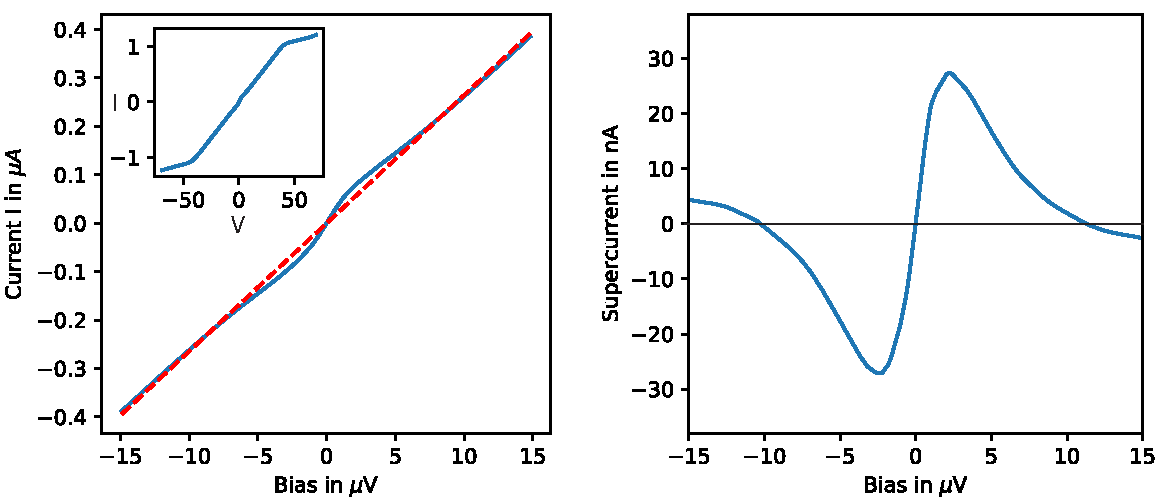
\includegraphics[width=0.89\linewidth]{fig/subtraction.pdf}
	\caption{\sffamily \, Experimentally measured IV-curve (left) and supercurrent
	contribution (right) that remains after subtracting the red-dashed
linear contribution.}
\label{fig:subtraction}
\end{figure}


\end{block}



\end{column} % End of the second column

\begin{column}{\sepwid}\end{column} % Empty spacer column

\begin{column}{\onecolwid} % The third column


\begin{figure}
	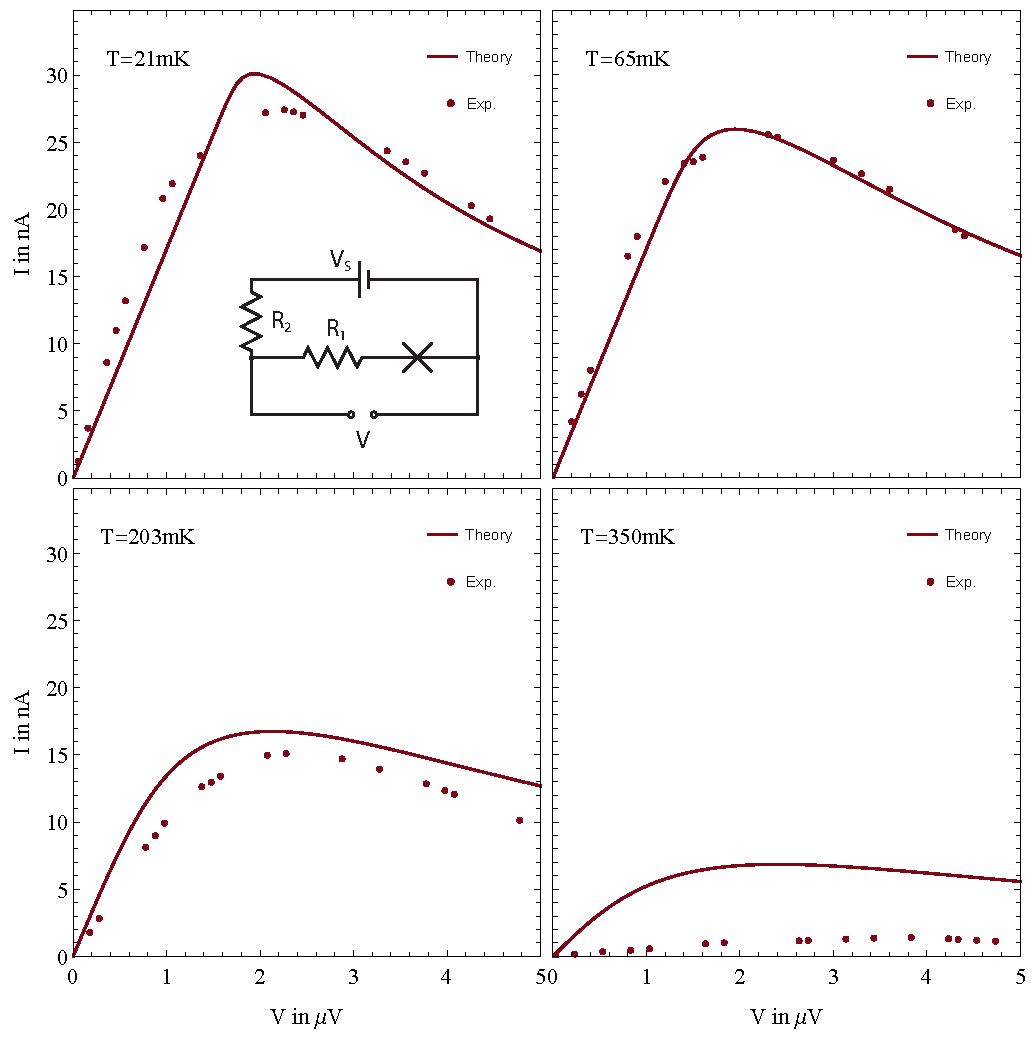
\includegraphics[width=0.93\linewidth]{fig/fig_fit2.pdf}
	\caption{\sffamily \, Experimentally measured IV curves (dots) at various
	temperatures agree well with the model Eq. \ref{eqn:zilberman} (red
	lines) for a
wide range of temperatures. Fit parameters are $I_0=\SI{35}{\nano\ampere}$,
$R_1=\SI{59}{\ohm}$, $R_2=\SI{88}{\ohm}$. The effective circuit is depicted in
the inset.}
\label{fig:fits}
\end{figure}

\begin{block}{Magnetic field dependence}
\begin{figure}
	\includegraphics[width=0.63\linewidth]{fig/mag_fit.pdf}
	\caption{\sffamily \, Simulated Fraunhofer magnetic field dependence of the
	differential conductance in good agreement to bottom left panel of Fig.
\ref{fig:exp}.}
\label{fig:magfit}
\end{figure}

Assuming a diffusive Josephson junction, the magnetic field dependence of the supercurrent follows the Fraunhofer
interference pattern
\begin{eqnarray*}
	I_0(\Phi) = I_0 \left|\frac{\sin(\pi\Phi/\Phi_0)}{\pi\Phi/\Phi_0}\right|
	\,.
\end{eqnarray*}
Figure \ref{fig:magfit} shows the resulting simulated differential conductance assuming a
junction area of 4\text{$\mu m^2$}, consistent with the
experimental geometry. The result is in good agreement to the experimental
data.

\end{block}

%----------------------------------------------------------------------------------------
%	CONCLUSION
%----------------------------------------------------------------------------------------
\begin{block}{Conclusion}
In summary, we report the observation of a large ZBCP in junction structures made of
normal metal (Ti/Au) – Dirac semimetal (Cd$_3$As$_2$) – conventional
superconductor (Al). Our detailed analyses suggest that this large ZBCP 
is due to the existence of a supercurrent between two far-separated
superconducting Al electrodes. Our results thus call for extreme caution when
assigning a large ZBCP to the MZM origin, especially when the width of the ZBCP
is below $3.5k_B T$.  
\end{block}



%----------------------------------------------------------------------------------------
%	REFERENCES
%----------------------------------------------------------------------------------------

\begin{block}{References}

\nocite{*} % Insert publications even if they are not cited in the poster
\small{\bibliographystyle{unsrt}
\bibliography{lit}\vspace{0.75in}}

\end{block}


%----------------------------------------------------------------------------------------

\end{column} % End of the third column

\end{columns} % End of all the columns in the poster

\end{frame} % End of the enclosing frame

\end{document}
